\section{Tensor de Tens\~ao}
\label{tensor_tens}

A resist\^encia que um material tem a sofrer deforma\c{c}\~oes
\'e causada por for\c{c}as chamadas de {\it
tens\~oes internas}. Assim, no estado sem deforma\c{c}\~ao,
essas for\c{c}as s\~ao nulas. Elas aparecem ap\'os a aplica\cao\
da for\c{c}a causadora da deforma\cao\ e tendem a preveni-la.
As tens\~oes internas existem somente entre part\'iculas vizinhas
do material, que est\~ao em contato direto. Por esse motivo,
s\~ao tamb\'em chamadas de for\c{c}as de contato.
O raio de a\c{c}\~ao dessas for\c{c}as \'e muito
pequeno. Podemos pensar que essas for\c{c}as agem atrav\'es de uma
superf\'{\i}cie ``imagin\'aria'', dividindo um elemento de volume
do corpo deformado do restante deste. Por causa disto, as tens\~oes
internas tamb\'em s\~ao conhecidas como {\it for\c{c}as de
superf\'{\i}cie}. Um exemplo desse tipo de for\c{c}a \'e a press\~ao
hidrost\'atica.

O elemento de volume considerado tamb\'em pode ser afetado por
for\c{c}as com raio de a\c{c}\~ao maior, como \'e o caso das
for\c{c}as gravitacional e eletromagn\'etica. Uma vez que essas
for\c{c}as, geralmente, s\~ao proporcionais ao volume do material,
elas s\~ao chamadas de for\c{c}as de volume ou de corpo. Uma fonte
s\'ismica tamb\'em \'e um exemplo de uma for\c{c}a de volume.

Vamos considerar um elemento de volume $\Delta V$, de um material
deformado interceptado por uma superf\'{\i}cie $\Delta S$ t\~ao
pequena, que as for\c{c}as de superf\'{\i}cie agindo sobre $\Delta
S$ podem ser substitu\'{\i}das por uma for\c{c}a equivalente
$\Delta \vec{T}$ agindo sobre $\Delta S$. Definimos ent\~ao,
\begin{equation}
\vec{T} = \lim_{\Delta S \rightarrow 0} {\Delta \vec{T} / \Delta
S}\;, \end{equation} onde $\vec{T}$ \'e o {\it vetor de tens\~ao}
ou {\it tra\c{c}\~ao}. Daqui por diante, quando tratarmos sobre
tens\~ao, estaremos tratando da densidade das for\c{c}as superficiais.

A tra\c{c}\~ao $\vec{T}$ depende da orienta\c{c}\~ao da
superf\'{\i}cie $\Delta S$ num dado ponto. Vamos ent\~ao denotar a
tra\c{c}\~ao que age sobre uma superf\'{\i}cie $\Delta S$ com
normal unit\'aria $\vec{n}$ por $\vec{T}(\vec{n})$. Pelo
princ\'{\i}pio da a\c{c}\~ao e rea\c{c}\~ao, a tra\c{c}\~ao
$\vec{T}(-\vec{n})$ agindo no outro lado da superf\'{\i}cie
$\Delta S$ deve ser de mesma intensidade, mas orienta\cao\ oposta
\begin{equation}
\vec{T}(-\vec{n})=-\vec{T}(\vec{n})\;.
\end{equation}

A tra\c{c}\~ao geralmente n\~ao coincide com a dire\c{c}\~ao da
normal $\vec{n}$. Por\'em, ela pode ser projetada na normal e
na superf\'icie. A componente de $\vec{T}(\vec{n})$ na normal
$\vec{n}$ \'e chamada {\it tens\~ao} normal, quando $\vec{T}(\vec{n})$
tende a separar as duas partes do elemento de volume, ou {\it
press\~ao} no caso contr\'ario. Os componentes tangentes
a superf\'icie $\Delta S$ s\~ao chamados de tens\~ao de cisalhamento.



Vamos introduzir as componentes de tens\~ao $\tau_{ij}$ como as
componentes da tra\c{c}\~ao agindo sobre um elemento de
superf\'{\i}cie, cuja normal est\'a ao longo do eixo $x_i$, isto
\'e, $\tau_{ij}=T_j(\vec{n}_i)$, onde $\vec{n}_i$ \'e o vetor normal ao
plano de coordenadas perpendicular ao eixo $x_i$. Vamos tentar determinar a
rela\c{c}\~ao entre a tra\c{c}\~ao $T_i(\vec{n})$ e a componente
de tens\~ao $\tau_{ij}$. Consideremos nosso elemento de volume
$\Delta V$ como sendo um tetraedro limitado pela superf\'{\i}cie
$\Delta S$, caracterizado pelas normais $\vec{n}_i$ e respectivas
superf\'{\i}cies $\Delta S_i$, nos planos perpendiculares aos
eixos de coordenadas, e $\vec{n}$ e $\Delta S_n$. 
\begin{figure}[!h]
\centering
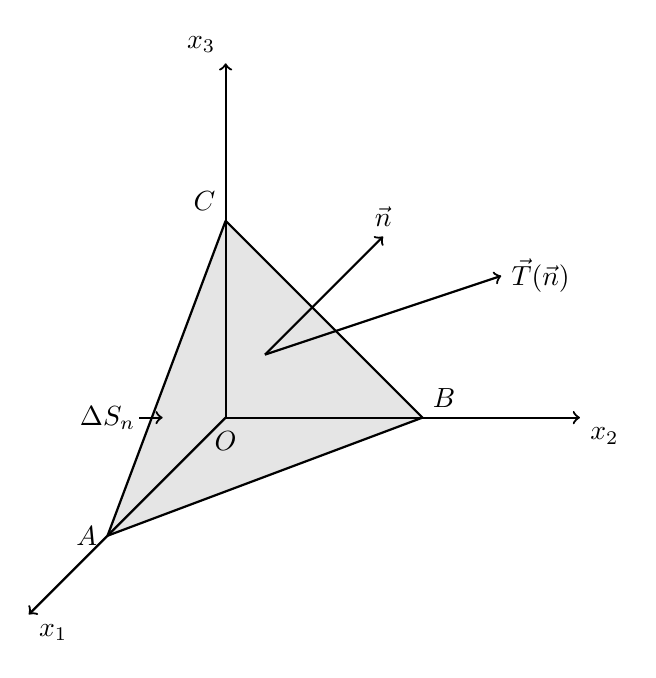
\begin{tikzpicture}
\fill[gray!20] (-1.5,-1.5) -- (0,2.5) -- (2.5,0); 
\draw[thick,->] (0,0) -- (4.5,0) node[anchor=north west] {$x_2$};
\draw[thick,->] (0,0) -- (0,4.5) node[anchor=south east] {$x_3$};
\draw[thick,->] (0,0) -- (-2.5,-2.5) node[anchor=north west] {$x_1$};
\draw[thick] (-1.5,-1.5) -- (0,2.5) node[anchor=south east] {$C$};
\draw[thick] (2.5,0) -- (-1.5,-1.5) node[anchor=east] {$A$};
\draw[thick] (0,2.5) -- (2.5,0) node[anchor=south west] {$B$};
%\fill[gray!50] (-1.5,-1.5) -- (0,2.5) -- (2.5,0); 
\draw[thick,->] (0.5,0.8) -- (2,2.3) node[anchor=south] {$\vec{n}$};
\draw[thick,->] (0.5,0.8) -- (3.5,1.8) node[anchor=west] {$\vec{T}(\vec{n})$};
\draw[thick,->] (-1.1,0) -- (-0.8,0); %node[anchor=east] {$\Delta S_n$};
\node[] at (-1.5,0) {$\Delta S_n$};
\node[] at (0,-0.3) {$O$};
\end{tikzpicture}
%Tetrahedron used to introduce the stress tensor. The surface dSn corresponds to the face ACB. The vector n is the normal to dSn and h is the distance from P to dSn. The faces BPC, APC, and APB are labeled dS1, dS2, dS3, respectively. The outer normal to dSi is the vector −ei 
\caption{Tetraedro usado para introduzir o tensor de tens\~ao. A superf\'icie $\Delta S_n$ corresponde a face ACB. O vetor $\vec{n}$ \'e a normal a $\Delta S_n$. As faces BOC, AOC e AOB s\~ao, respectivamente,  $\Delta S_1$, $\Delta S_2$ e $\Delta S_3$. A normal a $\Delta S_i$ \'e o vetor $\vec{n_i}$.}
\label{fig:tensor-tensao}
\end{figure}
Para um tetraedro suficientemente pequeno, as
for\c{c}as de corpo (proporcionais ao tamanho do volume) podem ser
desprezadas em compara\cao\ com as for\c{c}as de superf\'{\i}cie
(proporcionais ao tamanho da superf\'{\i}cie). Ent\~ao, a
condi\c{c}\~ao de equil\'{\i}brio para o tetraedro cont\'em somente
for\c{c}as de superf\'icie agindo no mesmo:
\begin{equation}
T_i(\vec{n}) \Delta S_n + T_i(-\vec{n}_1) \Delta S_1 +
T_i(-\vec{n}_2) \Delta S_2 + T_i(-\vec{n}_3) \Delta S_3 = 0 \;.
\end{equation}
Como $T_i(-\vec{n}_j)=-T_i(\vec{n}_j)$ e
$T_i(\vec{n}_j)=\tau_{ji}$, podemos reescrever a equa\c{c}\~ao
como
\begin{equation}
T_i(\vec{n}) \Delta S_n - \tau_{1i} \Delta S_1 - \tau_{2i} \Delta
S_2 - \tau_{3i} \Delta S_3 = 0 \;.
\end{equation}
Usando a seguinte rela\c{c}\~ao entre $\Delta S_n$ e $\Delta S_j$
\begin{equation}
\Delta S_j= (\vec{n} \cdot \vec{n}_j) \Delta S_n = \vec {n}_j \Delta S_n \;,
\end{equation}
na condi\c{c}\~ao de equil\'{\i}brio, obtemos
\begin{equation}
T_i(\vec{n}) = \tau_{ji} n_j \label{cond_equil}
\end{equation}


Esta rela\c{c}\~ao mostra que a tra\c{c}\~ao agindo numa
superf\'{\i}cie arbitr\'aria, especificada por uma normal
unit\'aria $\vec{n}$ pode ser expressada em termos das 9
componentes de tens\~ao $\tau_{ji}$. Considerando agora um  eixo
cartesiano rotacionado $x^{'}_i$ e escolhendo um eixo $x^{'}_k$ ao
longo da normal, podemos escrever
\begin{equation}
T^{'}_m(x^{'}_k) = \alpha_{mi} T_i(\vec{n}) = \alpha_{mi}
\tau_{ji} n_j = \alpha_{mi} \tau_{ji} \alpha_{lj} n^{'}_l =
\alpha_{mi} \alpha_{lj} \tau_{ji} \delta_{lk} = \alpha_{mi}
\alpha_{kj} \tau_{ji} \;.
\end{equation}

Isto quer dizer que $T^{'}_m(x^{'}_k)$ \'e a m-\'esima componente
da tra\c{c}\~ao agindo sobre o elemento de superf\'{\i}cie
perpendicular ao eixo $x^{'}_k$. $T^{'}_m(x^{'}_k)$ \'e ent\~ao
uma componente de tens\~ao $\tau^{'}_{km}$ e temos
\begin{equation}
\tau^{'}_{km} = \alpha_{kj} \alpha_{mi} \tau_{ji} \;.
\end{equation}
Mas isto \'e a equa\c{c}\~ao de transforma\c{c}\~ao de um tensor
de grau dois. Logo, as componentes de tens\~ao s\~ao elementos de
um tensor conhecido como {\it tensor de tens\~ao} $\tau_{ij}$.
Ele descreve o campo de tens\~ao em uma vizinhan\c{c}a de um certo ponto.





\subsection{Condi\c{c}\~ao de Equil\'{\i}brio}

Vamos considerar um pequeno volume $V$, em
equil\'{\i}brio est\'atico, de um material deformado.
O volume $V$ \'e limitado por uma
superf\'{\i}cie fechada $S$, caracterizada por uma normal unit\'aria
externa $\vec{n}$. Como o volume pode ser considerado r\'{\i}gido,
as condi\c{c}\~oes de equil\'{\i}brio de um corpo r\'{\i}gido
podem ser aplicadas a $V$. Para isso, \'e necess\'ario que a soma
de todas as for\c{c}as agindo sobre $V$ e de todos os seus momentos
desapare\c{c}am. Denotando a for\c{c}a de volume resultante por
$f_i$, escrevemos estas condi\c{c}\~oes como
\begin{equation}
\label{eq:equilib-for}
 \int \!\! \int \!\!  \int_V f_j dV + \int \!\! \int_S T_j
(\vec{n}) dS = 0 \;,
\end{equation}
\begin{equation}
\label{eq:equilib-momen}
 \int \!\! \int \!\!  \int_V \varepsilon_{ijk} x'_j f_k dV + \int \!\! \int_S
\varepsilon_{ijk} x'_j T_k (\vec{n}) dS = 0 \;,
\end{equation}
Essas s\~ao as condi\c{c}\~oes de equil\'ibrio na forma integral.
Em ambas as equa\c{c}\~oes acima, o
s\'{\i}mbolo $x'_i$ denota o vetor radial de um ponto deslocado do
volume $V$ nas coordenadas de $Lagrange$, $x'_i = x_i+u_i$. Os
argumentos das for\c{c}as $f_i$ e $T_i (\vec{n})$ tamb\'em s\~ao
considerados nas coordenadas de Lagrange.

Usando o resultado (\ref{cond_equil}), podemos reescrever a
primeira condi\c{c}\~ao na forma
\begin{equation} \int \!\! \int
\!\! \int_V f_j dV + \int \!\! \int_S \tau_{ij}n_i dS = 0 \;.
\end{equation}
Aplicando agora o Teorema de Gauss na integral de superf\'{\i}cie,
obtemos
\begin{equation}
\int \!\! \int \!\!  \int_V (f_j + \partial \tau_{ij}/\partial x'_i
)dV= 0 \;. \label{cond_int}
\end{equation}
Como o integrando em (\ref{cond_int}) \'e uma fun\c{c}\~ao
cont\'{\i}nua nas vari\'aveis espaciais e o volume pode ser
escolhido arbitrariamente, podemos escrever para qualquer ponto do
volume deformado
\begin{equation}
f_j + \partial \tau_{ij}/\partial x'_i = 0 \;.
\label{eq_equi_back}
\end{equation}

%
Assumindo que o termo $\partial \tau_{ij}/\partial x'_k$ \'e pequeno e
que seu produto com $\partial u_i/\partial x_j$ \'e
desprez\'{\i}vel, temos
\begin{equation}
\frac {\partial \tau_{ij}}{\partial x_i} = \frac {\partial
\tau_{ij}}{\partial x'_k} \frac {\partial x'_k}{\partial x_i}=\frac
{\partial \tau_{ij}}{\partial x'_k} \left(
\delta_{ik}+\frac{\partial u_k}{\partial x_i} \right) \approx \frac
{\partial \tau_{ij}}{\partial x'_i} \;. \label{eq_equi_back2}
\end{equation}

Podemos escrever
\begin{equation}
f_j + \tau_{ij,i} = 0 \;, \label{eq_equi_est}
\end{equation}
%
que \'e a {\it equa\c{c}\~ao de equil\'{\i}brio est\'atico} (na
forma diferencial) de um material deformado.

Agora, analogamente ao que foi feito para a condi\c{c}\~ao sobre
as for\c{c}as, fa\c{c}amos para a condi\c{c}\~ao sobre os
momentos, isto \'e, usando o resultado (\ref{cond_equil})
escrevemos a equa\cao\ \ref{eq:equilib-momen} como
\begin{equation}
\int \!\! \int \!\! \int_V \varepsilon_{ijk} x'_j f_k dV + \int
\!\! \int_S \varepsilon_{ijk} x'_j \tau_{lk}n_l dS = 0 \;.
\label{cond_moment}
\end{equation}
Aplicando o Teorema de Gauss na integral de superf\'{\i}cie,
obtemos
\begin{equation}
\begin{array}{rcl}
\int \!\! \int_S \varepsilon_{ijk} x'_j \tau_{lk}n_l dS &=& \int
\!\! \int \!\! \int_V  \varepsilon_{ijk} \partial (x'_j
\tau_{lk})/\partial x'_l dV  \\
&& \int \!\! \int \!\! \int_V  \varepsilon_{ijk} (\delta_{lj} \tau_{lk} + x'_j \tau_{lk,l}) dV \\
&& \int \!\! \int \!\! \int_V  \varepsilon_{ijk} \tau_{jk} dV -
\int \!\! \int \!\! \int_V  \varepsilon_{ijk} x'_j f_k dV \;.
\end{array}
\end{equation}
Na \'ultima passagem, usamos a equa\c{c}\~ao (\ref{eq_equi_est}).
Ent\~ao, a equa\c{c}\~ao (\ref{cond_moment}) toma a forma
\begin{equation}
\int \!\! \int \!\! \int_V  \varepsilon_{ijk} \tau_{jk} dV =0\;.
\label{cond_moment1}
\end{equation}
Como $V$ \'e arbitr\'ario, podemos escrever para qualquer ponto do
material em equil\'{\i}brio
\begin{equation}
\varepsilon_{ijk} \tau_{jk}=0\;.
\end{equation}
Usando as propriedades do s\'{\i}mbolo de {\it Levi-Civita},
obtemos
\begin{equation}
\tau_{jk}-\tau_{kj}=0\;.
\end{equation}

Portanto, o {\it tensor de tens\~ao} \'e sim\'etrico. Logo, ele
pode ser especificado apenas por 6 componentes independentes.



\subsection{Equa\c{c}\~ao de Movimento}

A equa\c{c}\~ao (\ref{eq_equi_est}) descreve um equil\'{\i}brio
est\'atico. Para obter as equa\c{c}\~oes de movimento
(equa\c{c}\~ao din\^amica), podemos usar o princ\'{\i}pio de
d'Alembert. Conforme este, equa\c{c}\~oes est\'aticas tornam-se
din\^amicas quando adicionamos for\c{c}as inerciais \`as
equa\c{c}\~oes est\'aticas.

A densidade de for\c{c}a inercial pode ser escrita como $\rho
\partial^2u_i / \partial t^2$. Assim, a equa\c{c}\~ao din\^amica toma a
forma
\begin{equation}
\tilde{f}_j + \tilde{\tau}_{ij,i} = \rho \frac{
\partial^2u_i }{ \partial t^2 }\;,
\label{eq_dinam_ger}
\end{equation}
onde as quantidades com tilda representam as for\cas\ e tens\oes\ do
estado din\^amico. Desde j\'a, podemos observar que somente for\cas\ e
tens\oes\ al\'em das do equil\ibrio\ influenciam a propaga\c{c}\~ao de
ondas. Isto se conclui pelo fato de que podemos subtra\ir\ a equa\cao\
(\ref{eq_equi_est}) da equa\cao\ (\ref{eq_dinam_ger}), obtendo
\begin{equation}
(\tilde{f}_j -f_j) + (\tilde{\tau}_{ij}-\tau_{ij})_{,i} = \rho \frac{
\partial^2u_i }{ \partial t^2 }\;,
\label{eq_dinam_pur}
\end{equation}
Simplificando a nota\cao, denotamos daqui adiante as diferen\cas\ das
for\cas\ din\^amicas de do equil\ibrio\ por $f_i$ e $\tau_{ij}$,
respectivamente, assim podendo escrever equa\cao\ (\ref{eq_dinam_pur})
como
\begin{equation}
f_j + \tau_{ij,i} = \rho \frac{
\partial^2u_i }{ \partial t^2 }\;,
\label{eq_dinam}
\end{equation}
Esta \'e a {\it equa\c{c}\~ao de movimento}, que \'e a equa\c{c}\~ao
b\'asica para descrever a propaga\c{c}\~ao de ondas. Mas antes de
resolv\'e-la, \'e necess\'ario especificar a equa\c{c}\~ao em termos do
deslocamento $u_i$. Para isto, o pr\'oximo estudo vai nos levar a uma
rela\c{c}\~ao entre tens\~ao e tra\c{c}\~ao.



\subsection{Tens\~oes Quadr\'aticas}

Uma superf\'{\i}cie de tens\~ao geralmente pode ser escrita na
forma
\begin{equation}
\tau_{ij} x_i x_j = \pm 1 \;.
\end{equation}
Express\oes\ deste tipo podem ser diagonalizado por uma rota\cao\ do
sistema de coordenadas. Obt\'em-se
\begin{equation}
\tau_{11}' {x'_1}^2 + \tau_{22}' {x'_2}^2 +
\tau_{33}' {x'_3}^2 = \pm 1 \;.
\end{equation}
Os eixos $x_i'$ destas quadr\'aticas s\~ao chamados de {\it
dire\c{c}\~oes principais da tens\~ao} e os valores
$\tau'_{11}$, $\tau'_{22}$ e $\tau'_{33}$ s\~ao as {\it
tens\~oes principais}. As {\it tens\~oes cisalhantes} $\tau'_{12}$,
$\tau'_{13}$ e $\tau'_{23}$ s\~ao nulas neste sistema
de coordenadas.



\section{Rela\c{c}\~oes Tens\~ao-Deslocamento}

Sabemos que a tens\~ao e o deslocamento s\~ao mutuamente
dependentes. Esta rela\c{c}\~ao depende do tipo de material e \'e,
portanto, uma importante caracter\'{\i}stica do material. De
acordo com os tipos de rela\c{c}\~oes, os materiais podem ser
chamados de el\'asticos, viscosos, viscoel\'asticos e pl\'asticos.
O foco dos estudos que seguem est\'a nos materiais el\'asticos, ou
seja, materiais que ap\'os terem uma carga removida, voltam ao seu
estado original como antes de terem a carga aplicada.

Vamos assumir que em cada ponto do meio, o tensor de tens\~ao \'e
unicamente determinado pelo deslocamento, isto \'e,
\begin{equation}
\tau_{ij}=\tau_{ij}(e_{kl}) \;.
\label{rel_tens_def}
\end{equation}
Assim, cada componente do tensor de tens\~ao depende geralmente de
cada componente do tensor de deslocamento, e essa depend\^encia
\'e geralmente n\~ao linear.

Por\'em, at\'e agora supomos que as deforma\coes\ s\ao\ pequenas
($e_{ij}\ll 1$) e negligenciamos termos de ordem maior do que um. Assim,
para manter a consist\^encia com o desenvolvimento at\'e agora, devemos
linearizar a rela\cao\ acima. Mais ainda, desde que consideramos
$\tau_{ij}$ como uma perturba\c{c}\~ao do estado inicial, n\'os podemos
colocar $\tau_{ij}(0)=0$. Desde modo, obtemos a chamada {\it Lei de Hooke
generalizada}
\begin{equation}
\tau_{ij}(x_m)=c_{ijkl}(x_m)e_{kl} (x_m) \;,
\label{lei_hooke}
\end{equation}
onde $c_{ijkl}$ s\~ao constantes de proporcionalidade, chamadas {\it
par\^ametros el\'asticos} ou {\it Tensor de Elasticidade}.

Deve se observar que a lineariza\cao\ que deu origem \`a Lei de Hooke
generalizada n\ao\ se justifica somente pela matem\'atica. Muitos
experimentos de elasticidade, como por exemplo o esticamento de um
haste, mostram na pr\'atica a exist\^encia de uma rela\cao\ linear entre
a deforma\cao\ de um corpo el\'astico e a tens\ao\ necess\'aria para
deform\'a-lo, pelo menos enquanto esta deforma\cao\ realmente \'e
el\'astica, i.e., depois da carga de tens\ao\ removida, o corpo volta
\`a sua forma original. Esta observa\cao\ de linearidade \'e conhecida
como {\em Lei de Hooke} e deu origem ao nome da rela\cao\
(\ref{lei_hooke}).

